
\documentclass[12pt]{article}

\usepackage{fancyhdr} 
\usepackage{lastpage} 
\usepackage{extramarks} 
\usepackage{graphicx,color}
\usepackage{anysize}
\usepackage{amsmath}
\usepackage{amssymb} 
\usepackage{natbib}
\usepackage{caption}
\usepackage{hyperref}
\usepackage{listings}
\usepackage{float}
\usepackage{xcolor}
\usepackage{enumitem}
\usepackage{booktabs}
\usepackage{longtable}
\pagecolor{white}

% Margins
\textwidth=6.5in
\setlength{\headheight}{15pt} 
\linespread{1.0} 

%%------------------------------------------------
%% Image and Listing code
%%------------------------------------------------
\newcommand{\includecode}[4]{\lstinputlisting[float, caption={[#1]#2}, captionpos=b, frame=single, label={#3}]{#4}}

\newcommand{\includescalefigure}[5]{
\begin{figure}[htb]
\centering
\includegraphics[width=#4\linewidth]{#5}
\captionsetup{width=.8\linewidth} 
\caption[#2]{#3}
\label{#1}
\end{figure}
}

\newcommand{\includefigure}[4]{
\begin{figure}[htb]
\centering
\includegraphics{#4}
\captionsetup{width=.8\linewidth} 
\caption[#2]{#3}
\label{#1}
\end{figure}
}

%%------------------------------------------------
%% Parameters
%%------------------------------------------------
\pagestyle{fancy}
\lhead{\teamName} % Top left header
\chead{\moduleCode\ - \assignmentTitle} % Top center header
\rhead{\firstxmark} % Top right header
\lfoot{\lastxmark} % Bottom left footer
\cfoot{} % Bottom center footer
\rfoot{Page\ \thepage\ of\ \pageref{LastPage}} % Bottom right footer
\renewcommand\headrulewidth{0.4pt} % Size of the header rule
\renewcommand\footrulewidth{0.4pt} % Size of the footer rule

\setlength\parindent{0pt}

% Project Info
\newcommand{\assignmentTitle}{Project Plan - HAB Detection System} 
\newcommand{\moduleCode}{COMP47250} 
\newcommand{\moduleName}{Team Software Project} 
\newcommand{\teamName}{Gradient\ Descent} 
\newcommand{\projectTitle}{HAB (Harmful Algal Bloom) Detection System}

% Team Members 
\newcommand{\memberOne}{Daniel Ilyin [18327256]}
\newcommand{\memberTwo}{Sagar Satish Poojary [24205485]}
\newcommand{\memberThree}{Dharmik Arvind Vara [24215287]}
\newcommand{\memberFour}{Karthika Garikapati [24206355]}
\newcommand{\memberFive}{Kruthi Jangam [24206846]}
\newcommand{\memberSix}{Roshan Palem [24209558]}

\date{}
\newcommand{\subsubsubsection}[1]{\paragraph{#1}\mbox{}\\}
\setcounter{secnumdepth}{4}
\setcounter{tocdepth}{4}

%%------------------------------------------------
%%	Title Page
%%------------------------------------------------
\title{
\vspace{-1in}
\begin{figure}[!ht]
\flushleft

\includegraphics[width=0.4\linewidth]{UCD.jpg}
\end{figure}
\vspace{-0.5cm}
\hrulefill \\
\vspace{0.5cm}
\textmd{\textbf{\moduleCode\ \moduleName}}\\
\textmd{\textbf{\assignmentTitle}}\\
\textmd{\textbf{Team: \teamName}}\\
\vspace{0.5cm}
\hrulefill \\
}
\author{
\textbf{Team Members:}\\
\memberOne\\
\memberTwo\\
\memberThree\\
\memberFour\\
\memberFive\\
\memberSix\\
}

%%------------------------------------------------
%% Document
%%------------------------------------------------
\begin{document}
%% Defaults for listings
\lstset{language=Python, captionpos=b, frame=single}
\captionsetup{width=.8\linewidth} 

\maketitle
\tableofcontents
\vspace{0.5in}

%%------------------------------------------------
\section{Project Objectives}

This project aims to develop a web-based Harmful Algal Bloom (HAB) detection and prediction system based on the HABNet architecture proposed by Hill et al. (2020). HABs pose significant risks to marine ecosystems, aquaculture operations, and public health, with traditional detection methods relying on periodic manual sampling that leads to delayed response times.

Our system will implement a spatiotemporal "datacube" approach combined with deep neural networks to achieve high-accuracy HAB detection and prediction capabilities. The primary objectives include:

\textbf{Core Technical Objectives:}
\begin{itemize}
    \item Develop an automated datacube generator for processing remote sensing data from MODIS-Aqua/Terra satellites and Sentinel-3 sensors
    \item Implement and train deep learning models (NASNet-Mobile backbone with LSTM) for HAB event classification
    \item Create a minimum viable reproduction achieving >90\% detection accuracy and ~80\% prediction accuracy
    \item Build a real-time web-based dashboard for HAB monitoring and prediction
\end{itemize}

\textbf{User-Centered Objectives:}
\begin{itemize}
    \item Provide marine biologists and environmental agencies with early warning capabilities (up to 8 days ahead)
    \item Enable aquaculture operators to implement timely mitigation measures
    \item Support public health officials in issuing timely advisories for recreational water use
\end{itemize}

Success will be measured through technical performance metrics (detection/prediction accuracy), user evaluation feedback, and system scalability demonstrations using cloud infrastructure.

%%------------------------------------------------
\section{Project Plan}

\subsection{Sprint Overview}
Our development follows an agile methodology with 2-week sprints aligned with project milestones:

\begin{longtable}{|p{2cm}|p{3cm}|p{8cm}|}
\hline
\textbf{Sprint} & \textbf{Dates} & \textbf{Deliverables \& Goals} \\
\hline
Sprint 1 & 20/5 - 2/6 & Team formation, environment setup, initial data source exploration \\
\hline
Sprint 2 & 3/6 - 16/6 & MVP development, basic datacube pipeline, simple classifier \\
\hline
Sprint 3 & 17/6 - 30/6 & Model training, interim presentation preparation, web interface prototype \\
\hline
Sprint 4 & 1/7 - 14/7 & Advanced model implementation, cloud deployment, user testing framework \\
\hline
Sprint 5 & 15/7 - 28/7 & System integration, performance optimization, comprehensive evaluation \\
\hline
Sprint 6 & 29/7 - 11/8 & Final testing, documentation, presentation preparation \\
\hline
Sprint 7 & 12/8 - 19/8 & Final report completion, system refinements \\
\hline
\end{longtable}

\subsection{Key Dates}
\begin{itemize}
    \item \textbf{9/6/2025:} Project Plan submission
    \item \textbf{23/6/2025:} Interim Presentation \& MVP Demo
    \item \textbf{4/8/2025:} Final Presentation \& Complete System Demo
    \item \textbf{19/8/2025:} Final Report submission
\end{itemize}

%%------------------------------------------------
\section{Roles}
%%------------------------------------------------
\begin{itemize}
  \item \textbf{Project Manager (Kruthi):} Tracks milestones, maintains sprint board, leads team syncs.
  \item \textbf{ML Lead (Roshan):} Leads model selection, training, and tuning.
  \item \textbf{Data Engineer (Karthika):} Manages dataset acquisition, cleaning, and ETL.
  \item \textbf{Frontend Developer (Dharmik):} Builds the Streamlit dashboard and integrates backend.
  \item \textbf{DevOps \& Cloud Lead (Daniel):} Sets up and maintains cloud infrastructure and deployment.
  \item \textbf{UX \& Testing Lead (Sagar):} Handles UI testing, SHAP analysis, and final user evaluations.
\end{itemize}



%%------------------------------------------------
\section{Architecture}
%%------------------------------------------------
\begin{figure}[H]
  \centering
  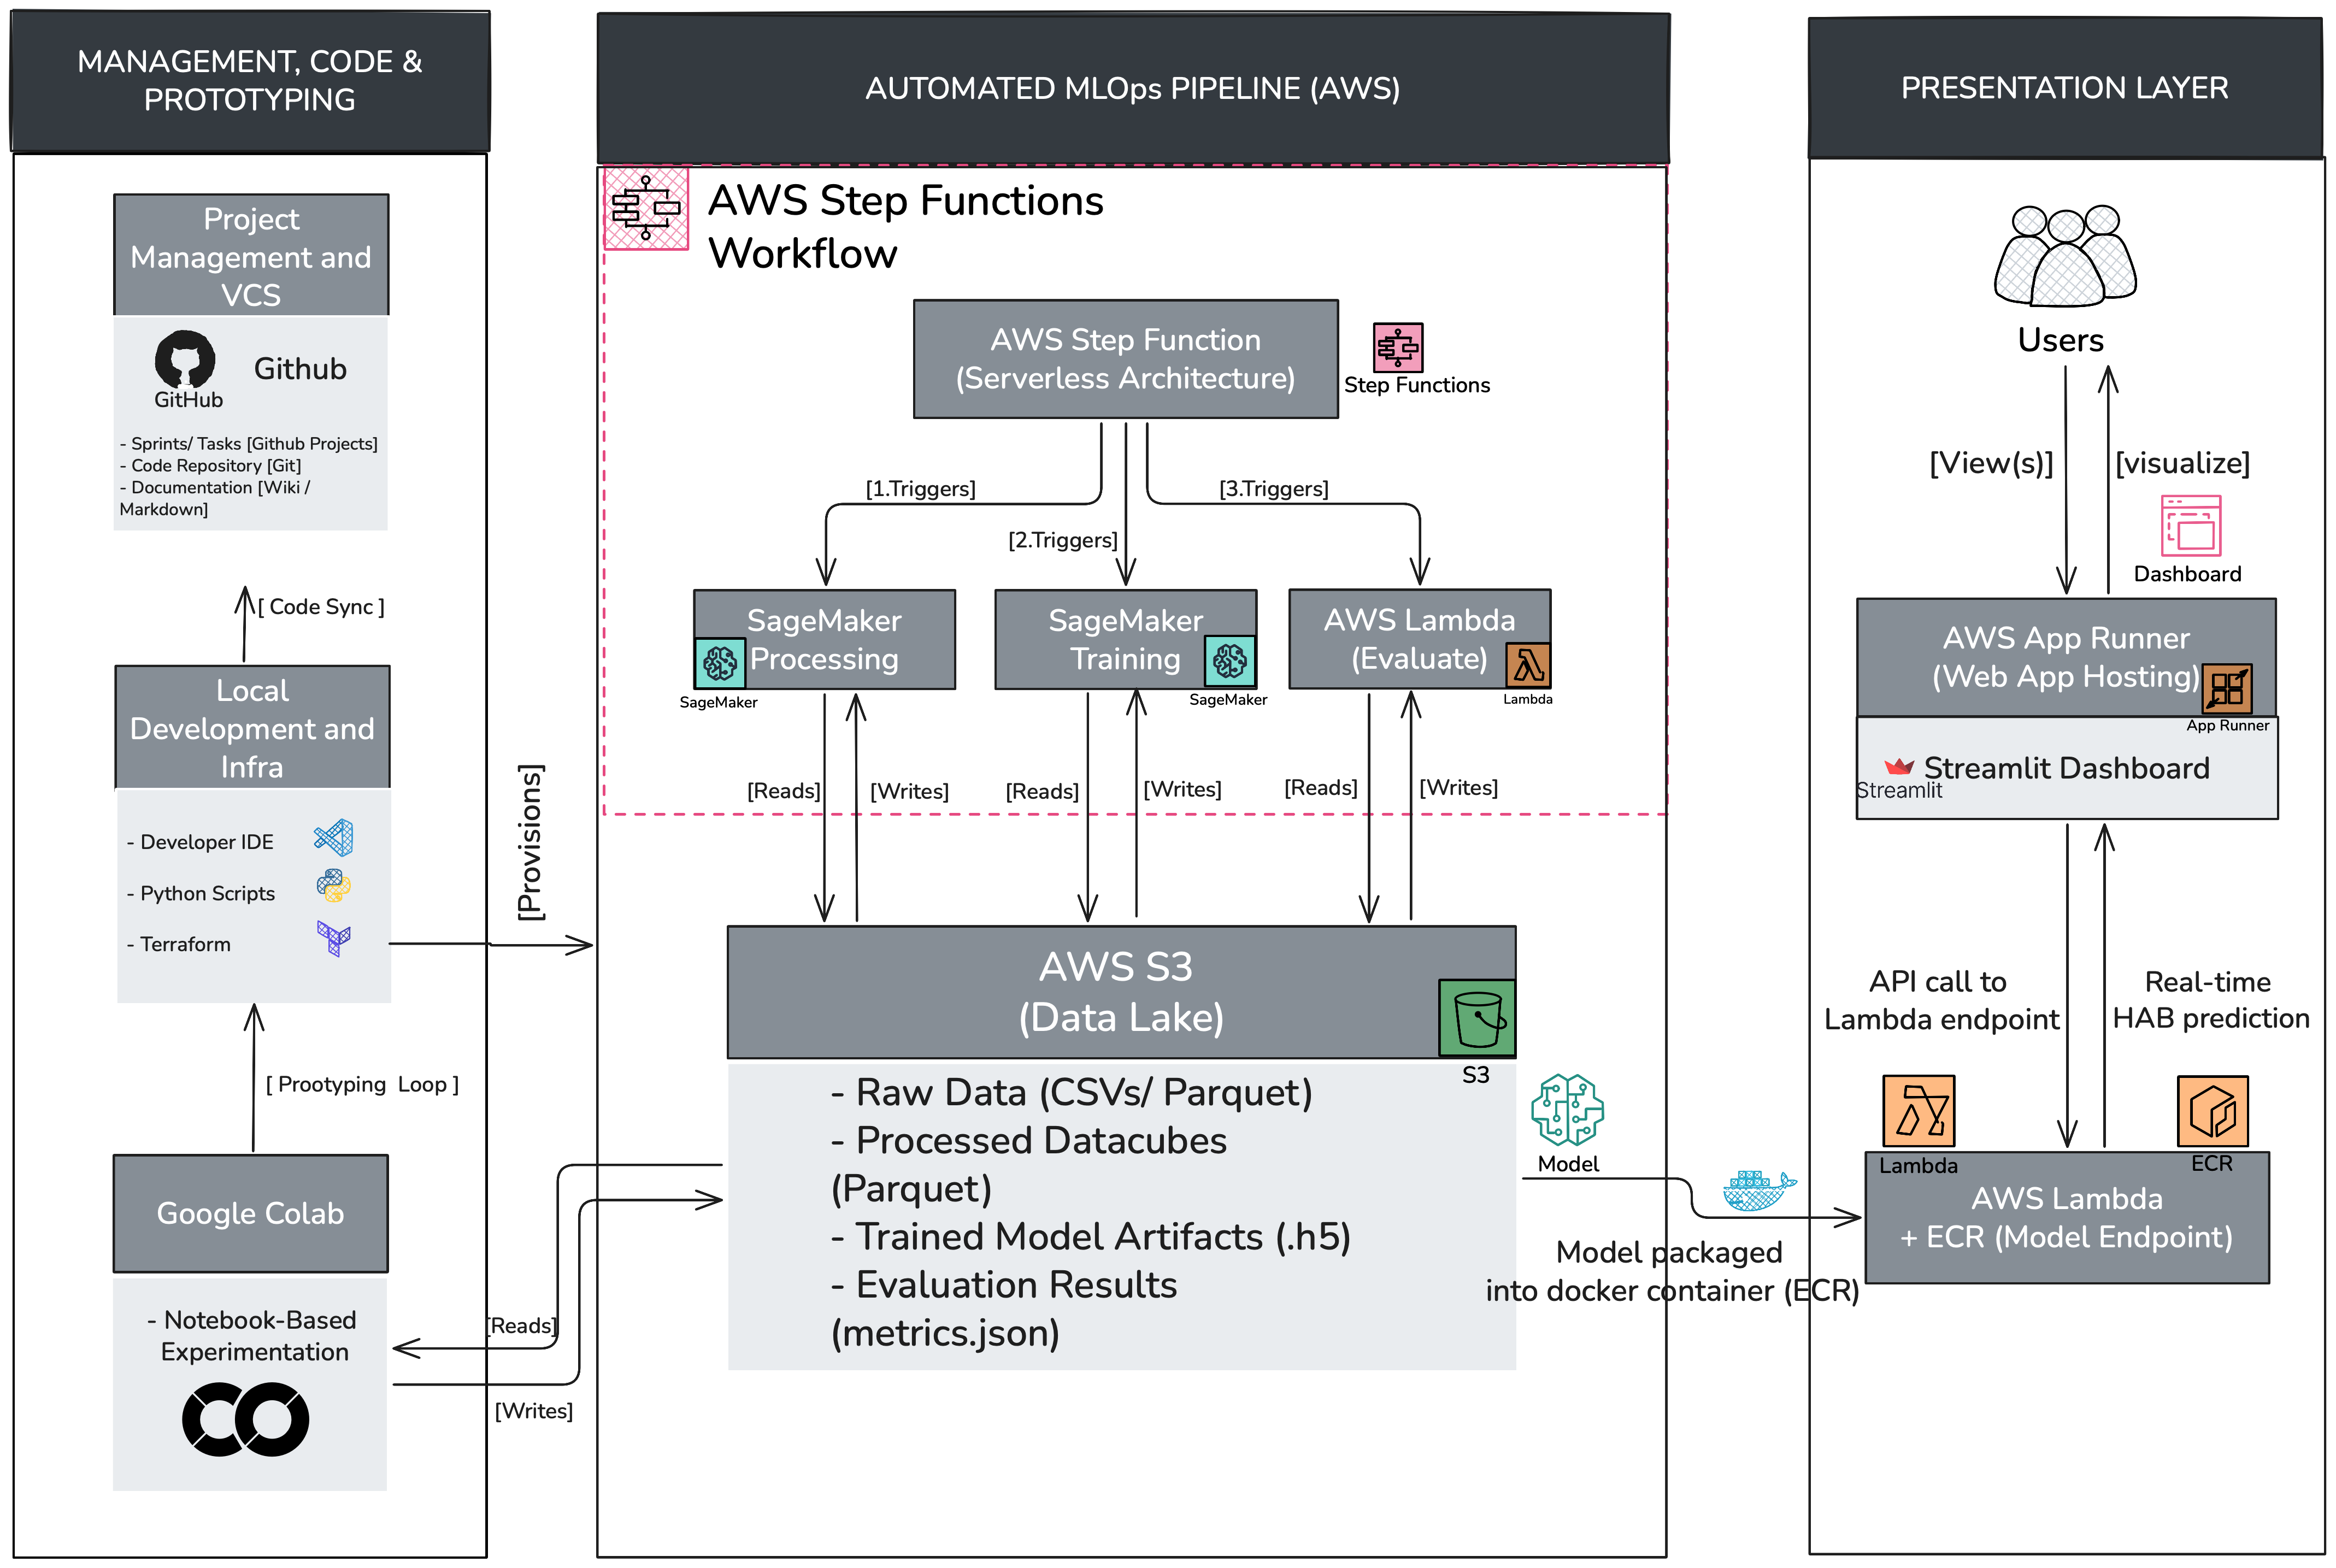
\includegraphics[width=\linewidth]{Project_Architecture_New.png}
  \caption{System architecture for HAB detection and prediction. The pipeline integrates local development, version control, and notebook experimentation with an automated AWS-based MLOps workflow using Step Functions, SageMaker, and Lambda. Outputs are stored in S3 and served through a Streamlit dashboard hosted on AWS App Runner for real-time HAB prediction.}
  \label{fig:hab-architecture}
\end{figure}


%%------------------------------------------------
\section{Data Plan}
%%------------------------------------------------
\subsection{Data Collection Strategy}

\subsubsection{Ground Truth Data Sources}
The primary source for labeled HAB events will be obtained from HAEDAT (Harmful Algal Event Database), which provides comprehensive data including:
\begin{itemize}
    \item Geographic coordinates of HAB events
    \item Temporal information (timestamps)
    \item Validated HAB event classifications
\end{itemize}

\subsubsection{Remote Sensing Image Data}
NASA MODIS satellite constellation serves as the primary source for remote sensing imagery:
\begin{itemize}
    \item \textbf{MODIS-Aqua}: Ocean color and temperature data
    \item \textbf{MODIS-Terra}: Land and atmospheric observations
\end{itemize}

\subsection{Data Preprocessing Pipeline}

The preprocessing workflow follows a systematic approach:

% \begin{equation}
\qquad $\text{Raw Data} \rightarrow \text{Resampling} \rightarrow \text{Feature Extraction} \rightarrow \text{Datacube Construction}$
% \end{equation}

\subsubsection{Image Preprocessing Steps}
\begin{itemize}
    \item \textbf{Raw Data Acquisition}: Collection of satellite imagery from MODIS sensors
    \item \textbf{Resampling}: Standardization of spatial and temporal resolution
    \item \textbf{Feature Extraction}: Identification of relevant spectral and spatial features
    \item \textbf{Datacube Construction}: Organization of multi-dimensional data arrays
\end{itemize}

\subsection{Data Structure and Labeling}

The dataset will be structured into two primary categories:
\begin{itemize}
    \item \textbf{Positive Samples}: Confirmed HAB events with corresponding satellite imagery
    \item \textbf{Negative Samples}: Non-HAB oceanic conditions for comparison
\end{itemize}

\subsubsection{Data Augmentation Strategy}
To enhance model robustness and increase training data diversity:
\begin{itemize}
    \item \textbf{Rotation}: Apply various rotational transformations
    \item \textbf{Flipping}: Horizontal and vertical image flipping
\end{itemize}

\subsection{Pretrained Model Implementation Plan}

\subsubsection{Primary Architecture}
The implementation will utilize a transfer learning approach:

% \begin{equation}
\qquad $\text{Pretrained CNN Backbone} \rightarrow \text{Feature Extraction} \rightarrow \text{Classification}$
% \end{equation}

\subsubsection{Pretrained Models}
Three candidate architectures will be evaluated:

\begin{itemize}
    \item \textbf{NASNet Mobile} (Recommended by original research)
    \item \textbf{EfficientNet-B0/B1} (Alternative approach)
    \item \textbf{ResNet-50} (Baseline comparison)
\end{itemize}

\subsubsection{Model Adaptation Strategies}
The adaptation process will follow a progressive approach:

\begin{itemize}
    \item \textbf{Feature Extraction}: Initial freezing of pretrained weights
    \item \textbf{Fine-tuning}: Gradual unfreezing of top layers
    \item \textbf{Layer Replacement}: Modification of final classification layers
\end{itemize}

\subsection{Training Strategy}

\subsubsection{Data Partitioning}
The dataset will be divided according to standard machine learning practices:

\begin{table}[H]
\centering
\begin{tabular}{@{}lc@{}}
\toprule
\textbf{Dataset Partition} & \textbf{Percentage} \\
\midrule
Training Set & 70\% \\
Validation Set & 10\% \\
Testing Set & 20\% \\
\bottomrule
\end{tabular}
% \caption{Dataset partitioning strategy}
% \label{tab:data_partition}
\end{table}

\subsubsection{Performance Evaluation}
Model performance will be monitored using established classification metrics:
\begin{itemize}
    \item \textbf{Precision}: $P = \frac{TP}{TP + FP}$
    \item \textbf{Recall}: $R = \frac{TP}{TP + FN}$
    \item \textbf{F1-Score}: $F_1 = 2 \cdot \frac{P \cdot R}{P + R}$
\end{itemize}

where $TP$, $FP$, and $FN$ represent true positives, false positives, and false negatives, respectively.



%%------------------------------------------------
\section{GitHub Repository}
%%------------------------------------------------
Our GitHub repository can be found at \href{https://github.com/danieli1245/Harmful-Algal-Bloom-Detection-System}{https://github.com/danieli1245/Harmful-Algal-Bloom-Detection-System}. Our repository demonstrates consistent team engagement with members contributing to project documentation, planning and initial development setup.

\subsection{Contribution Evidence}
\textbf{Commit Activity:}
Figure \ref{fig:commits} demonstrates the contributions from team members during the initial project setup phase. The repository shows meaningful commits including project structure setup, project plan creation, and demo material.

\begin{figure}[H]
\centering
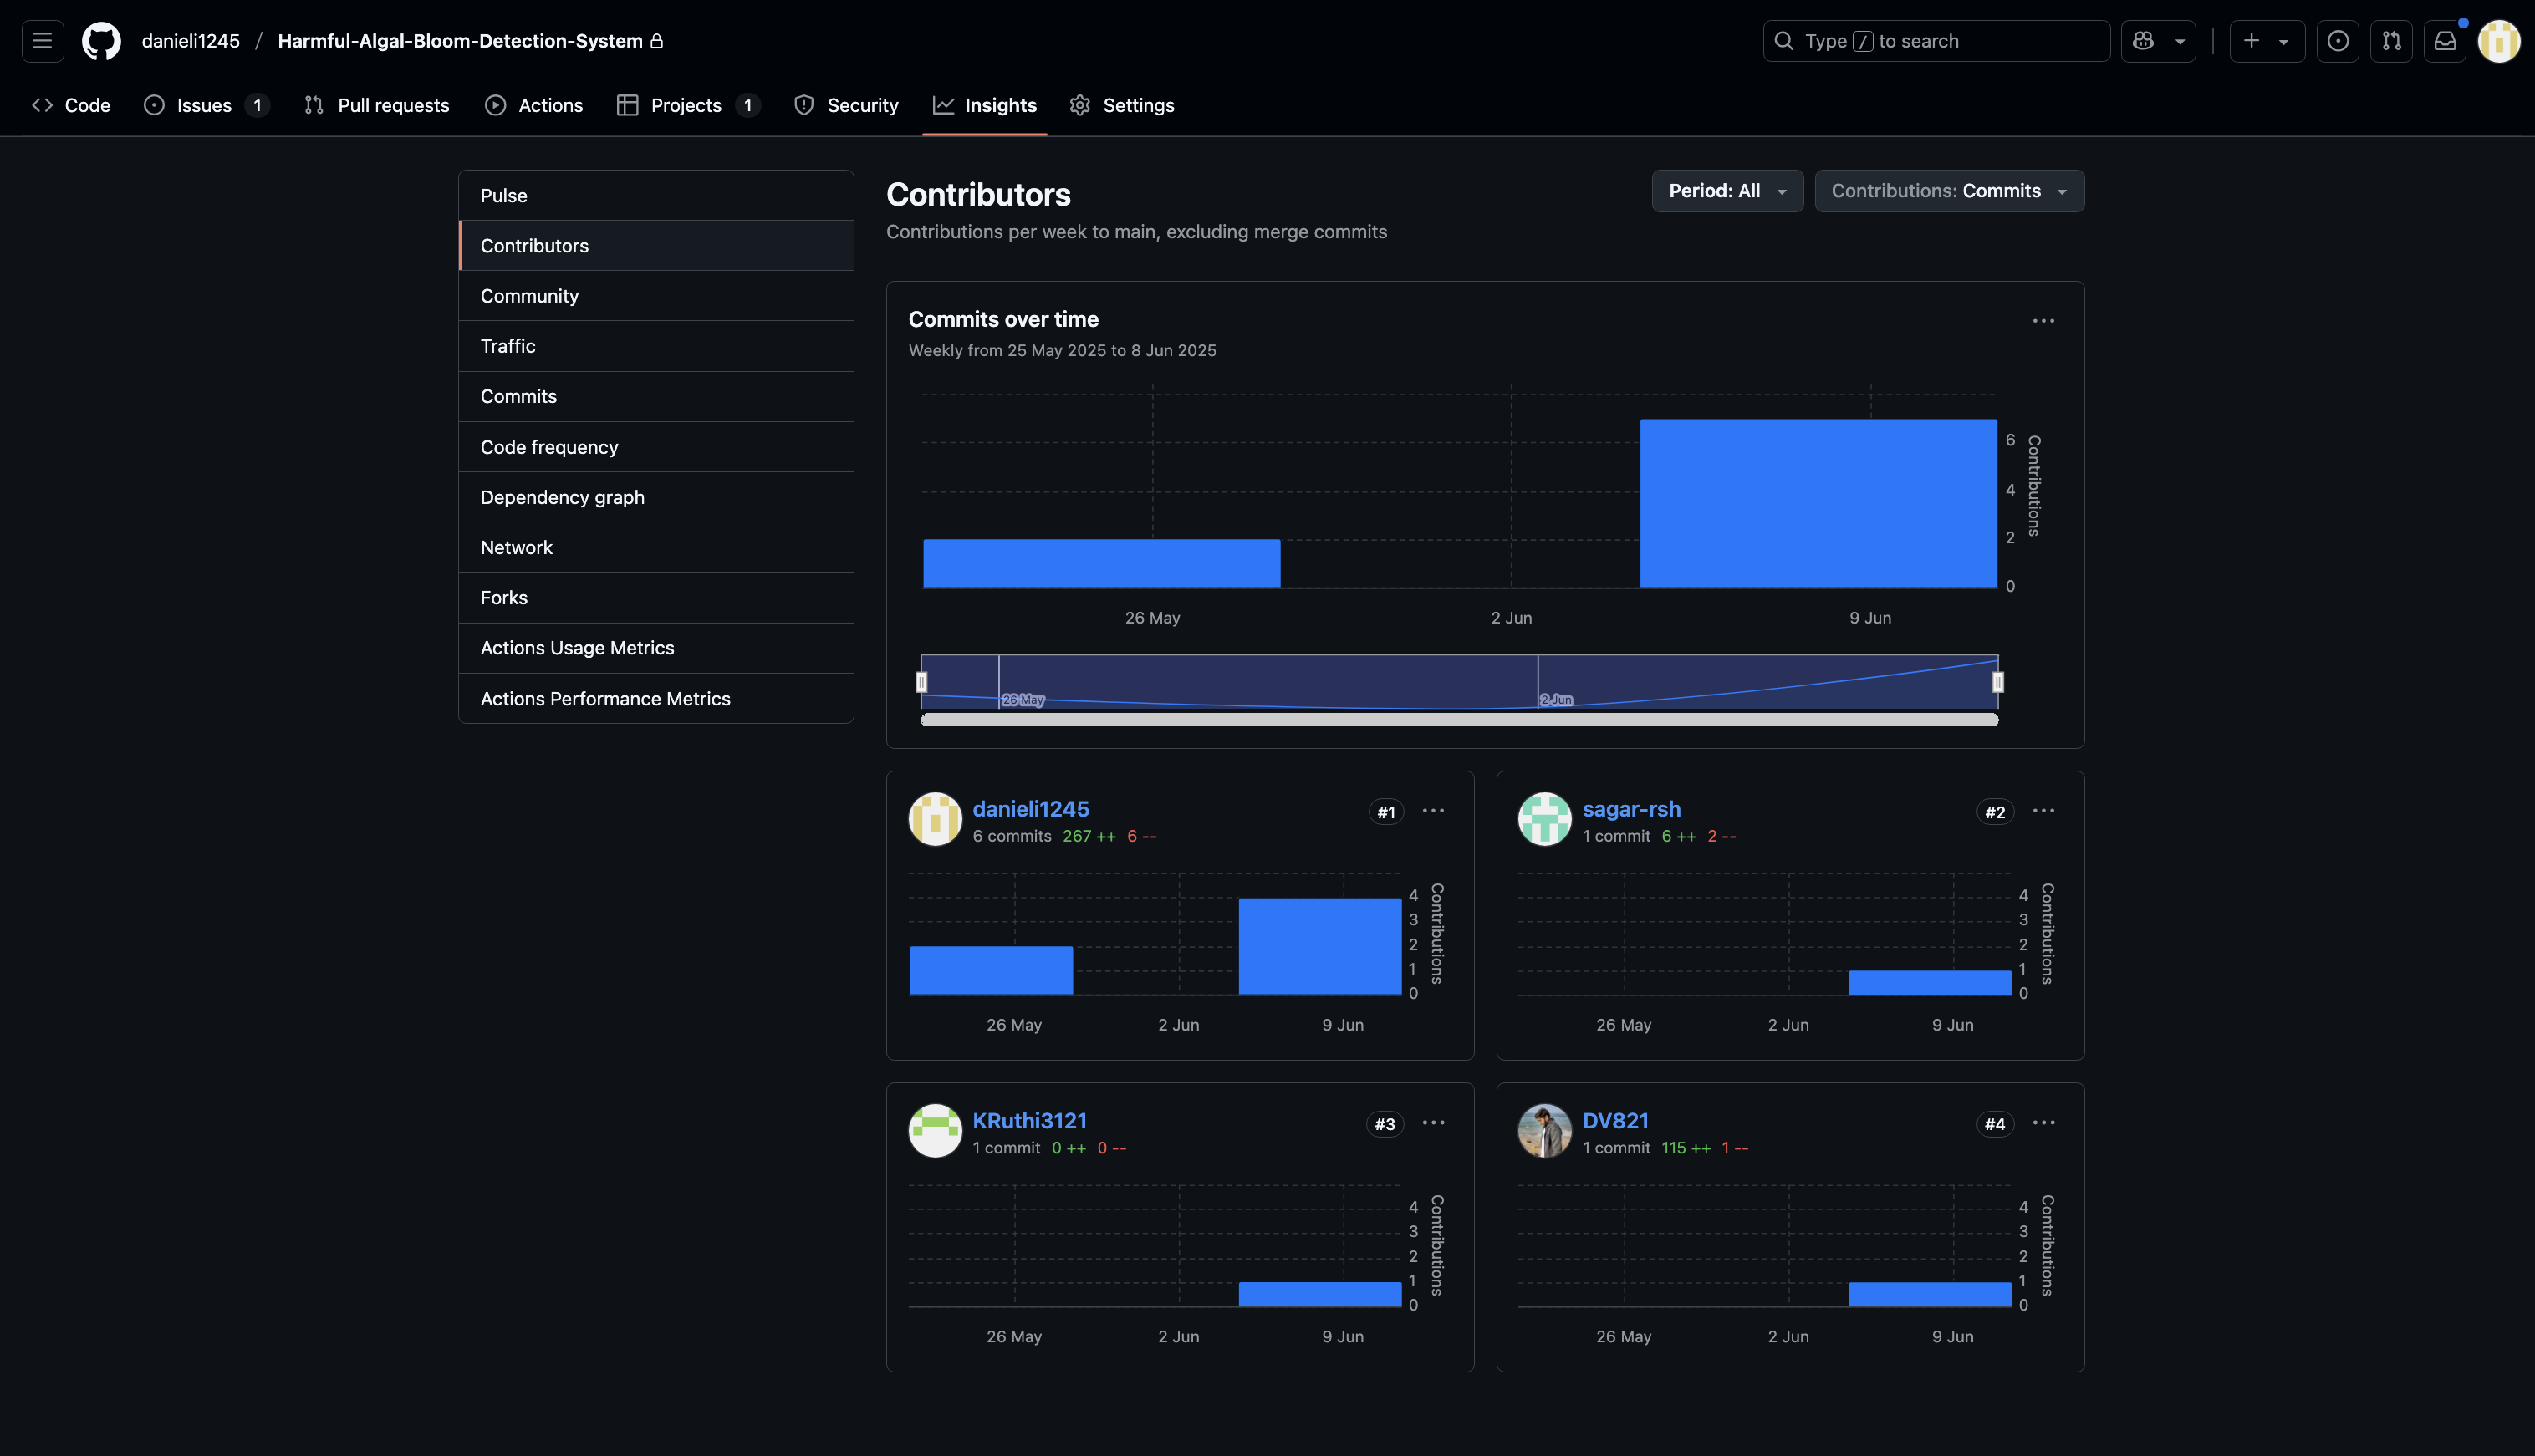
\includegraphics[width=0.9\linewidth]{Commits.png}
\captionsetup{width=.8\linewidth} 
\caption[GitHub Commits]{Evidence of regular commits from team members}
\label{fig:commits}
\end{figure}

\subsection{Team Meeting Documentation}
Regular team meetings are documented and minutes are created through zoom

\begin{figure}[H]
\centering
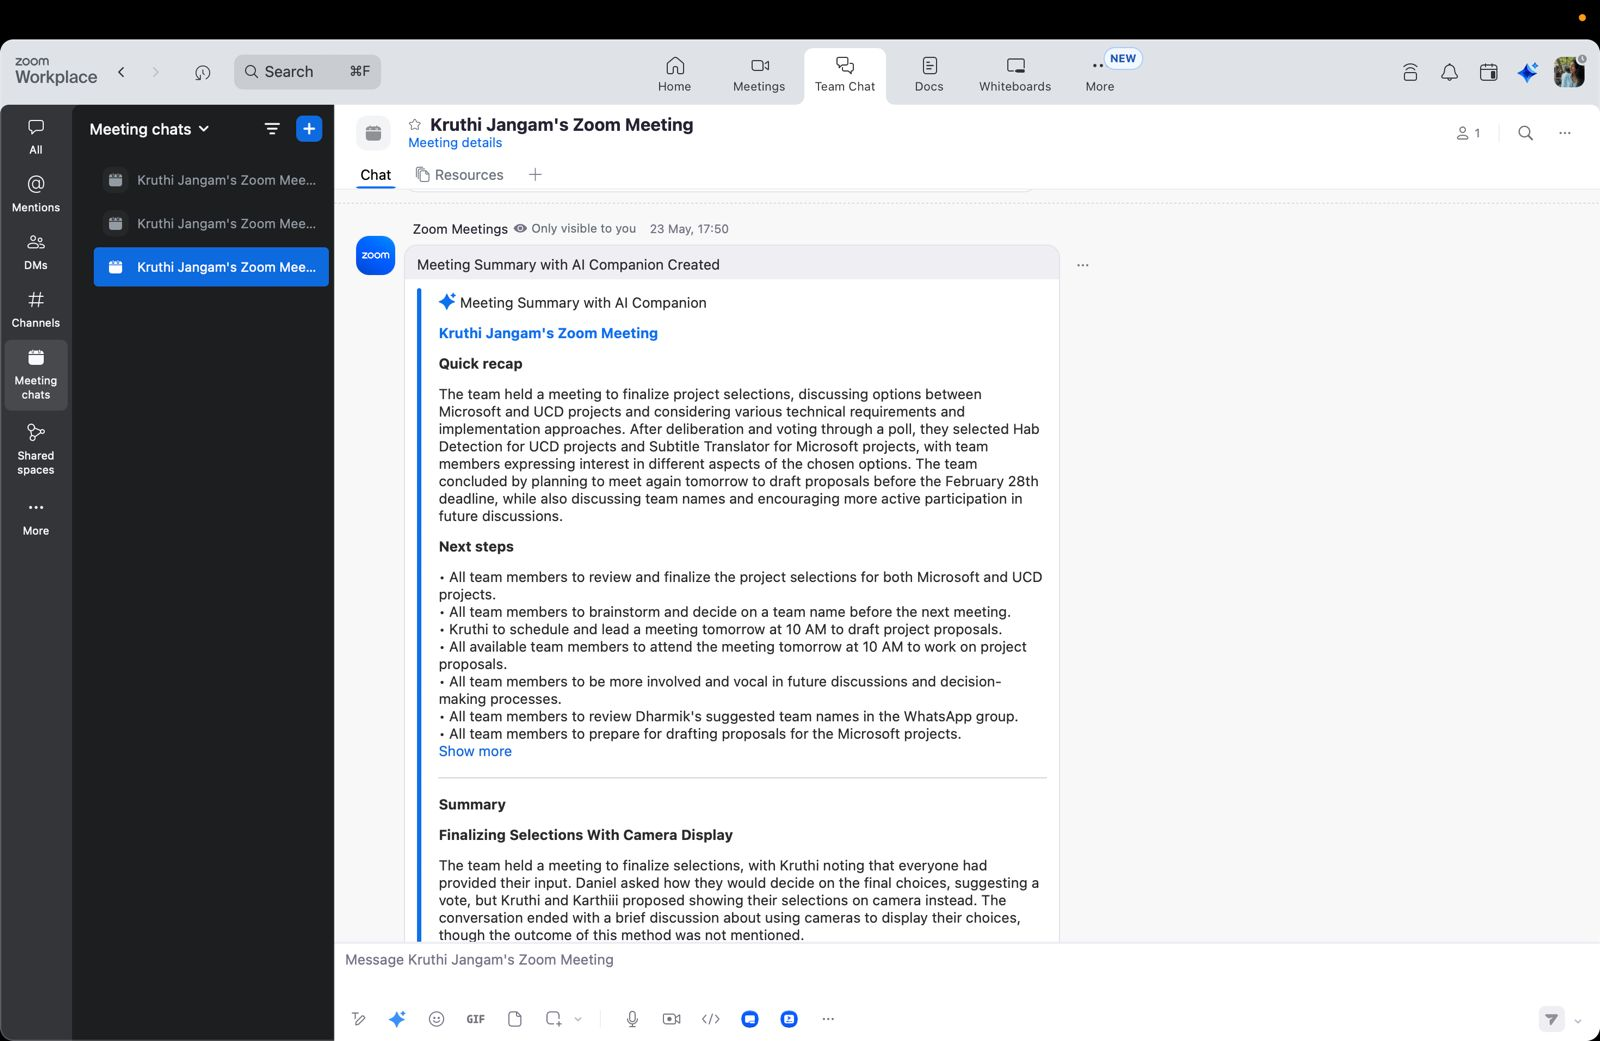
\includegraphics[width=0.8\linewidth]{Meetings.jpeg}
\captionsetup{width=.8\linewidth} 
\caption[Team Meeting Minutes]{Meeting minutes on zoom}
\label{fig:meeting}
\end{figure}

Then we upload the minutes to to our Github Projects dashboard

\begin{figure}[H]
\centering
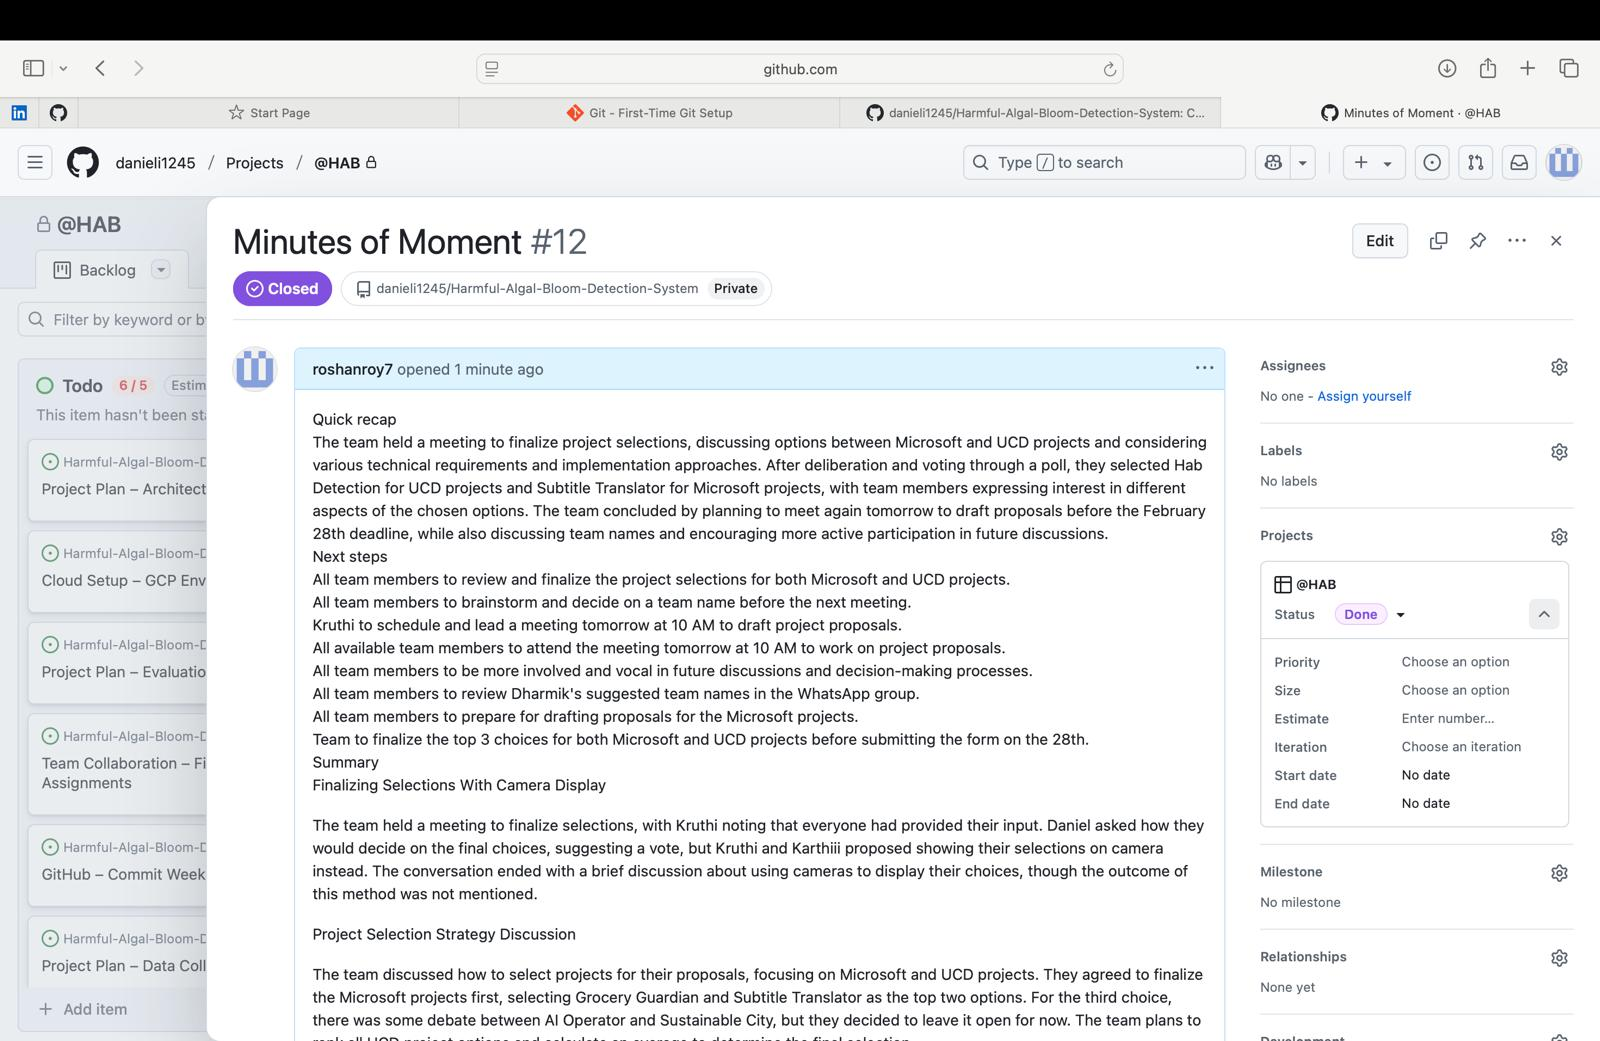
\includegraphics[width=0.8\linewidth]{Meetings2.jpeg}
\captionsetup{width=.8\linewidth} 
\caption[Team Meeting Minutes]{Meeting minutes on Github Project}
\label{fig:meeting}
\end{figure}


%%------------------------------------------------
\section{Team Management}
%%------------------------------------------------

\subsection{Meeting Format}

\textbf{Meeting Format:}
Our meetings are conducted via Zoom with structured agendas using Github Projects covering progress updates, blocker identification, and task assignments. All meetings are documented for future reference. We hold a main meeting every Monday, with other follow up meetings throughout the week, as needed.

\subsection{Meeting Documentation}
Regular team meetings are documented with full minutes capturing the key decisions and progress updates. Figure \ref{fig:meeting} shows our Zoom-based meeting format.

As referenced in Section 6, we maintain detailed meeting records that are then moved to our GitHub Projects dashboard for task tracking and sprint management (Figure \ref{fig:meeting2}).

\begin{figure}[H]
\centering
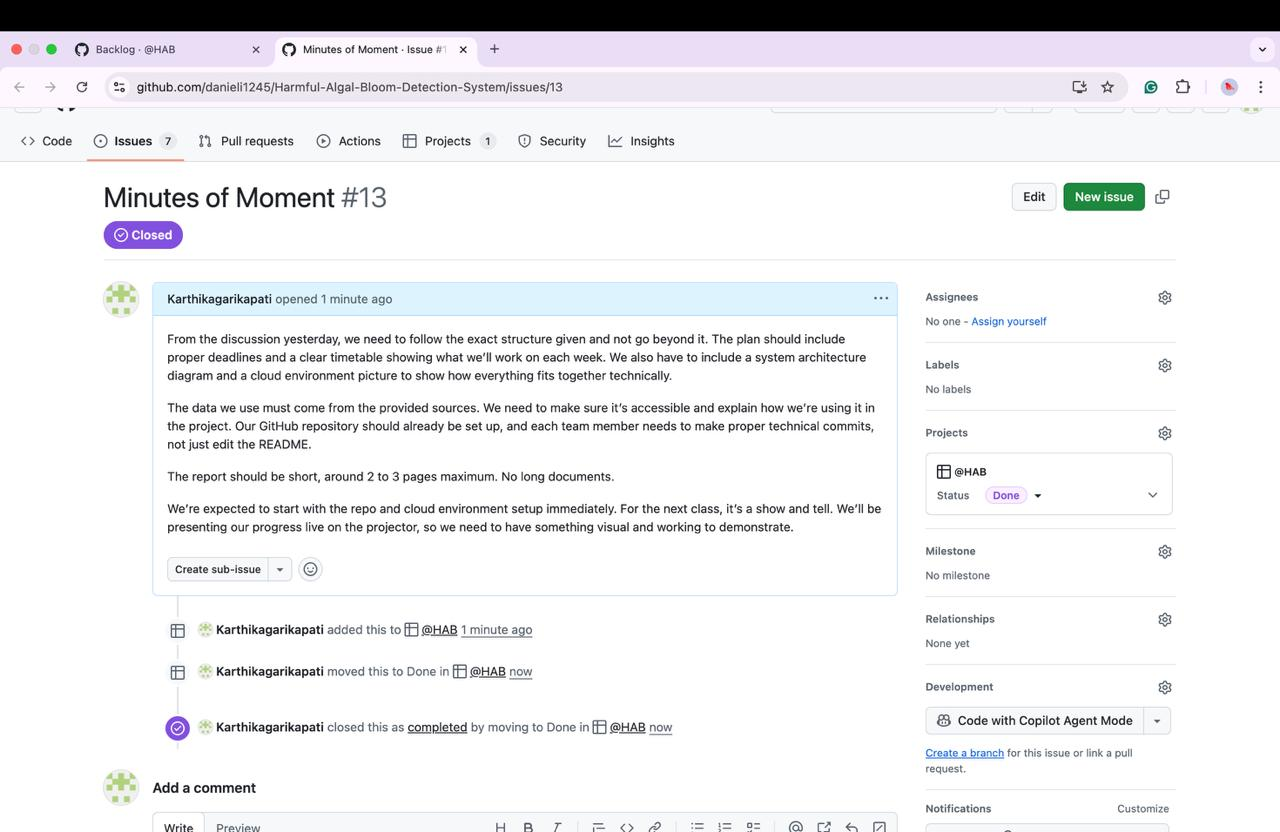
\includegraphics[width=0.8\linewidth]{Meetings3.jpeg}
\captionsetup{width=.8\linewidth} 
\caption[Additional Team Meeting]{Additional team meeting documentation}
\label{fig:meeting3}
\end{figure}

\subsection{Project Management Tools}
\textbf{GitHub Projects Dashboard:}
We use GitHub Projects as our primary project management tool for sprint planning and progress tracking. Figure \ref{fig:github-project} demonstrates our current board organisation with task categorisation and progress visibility.

\begin{figure}[H]
\centering
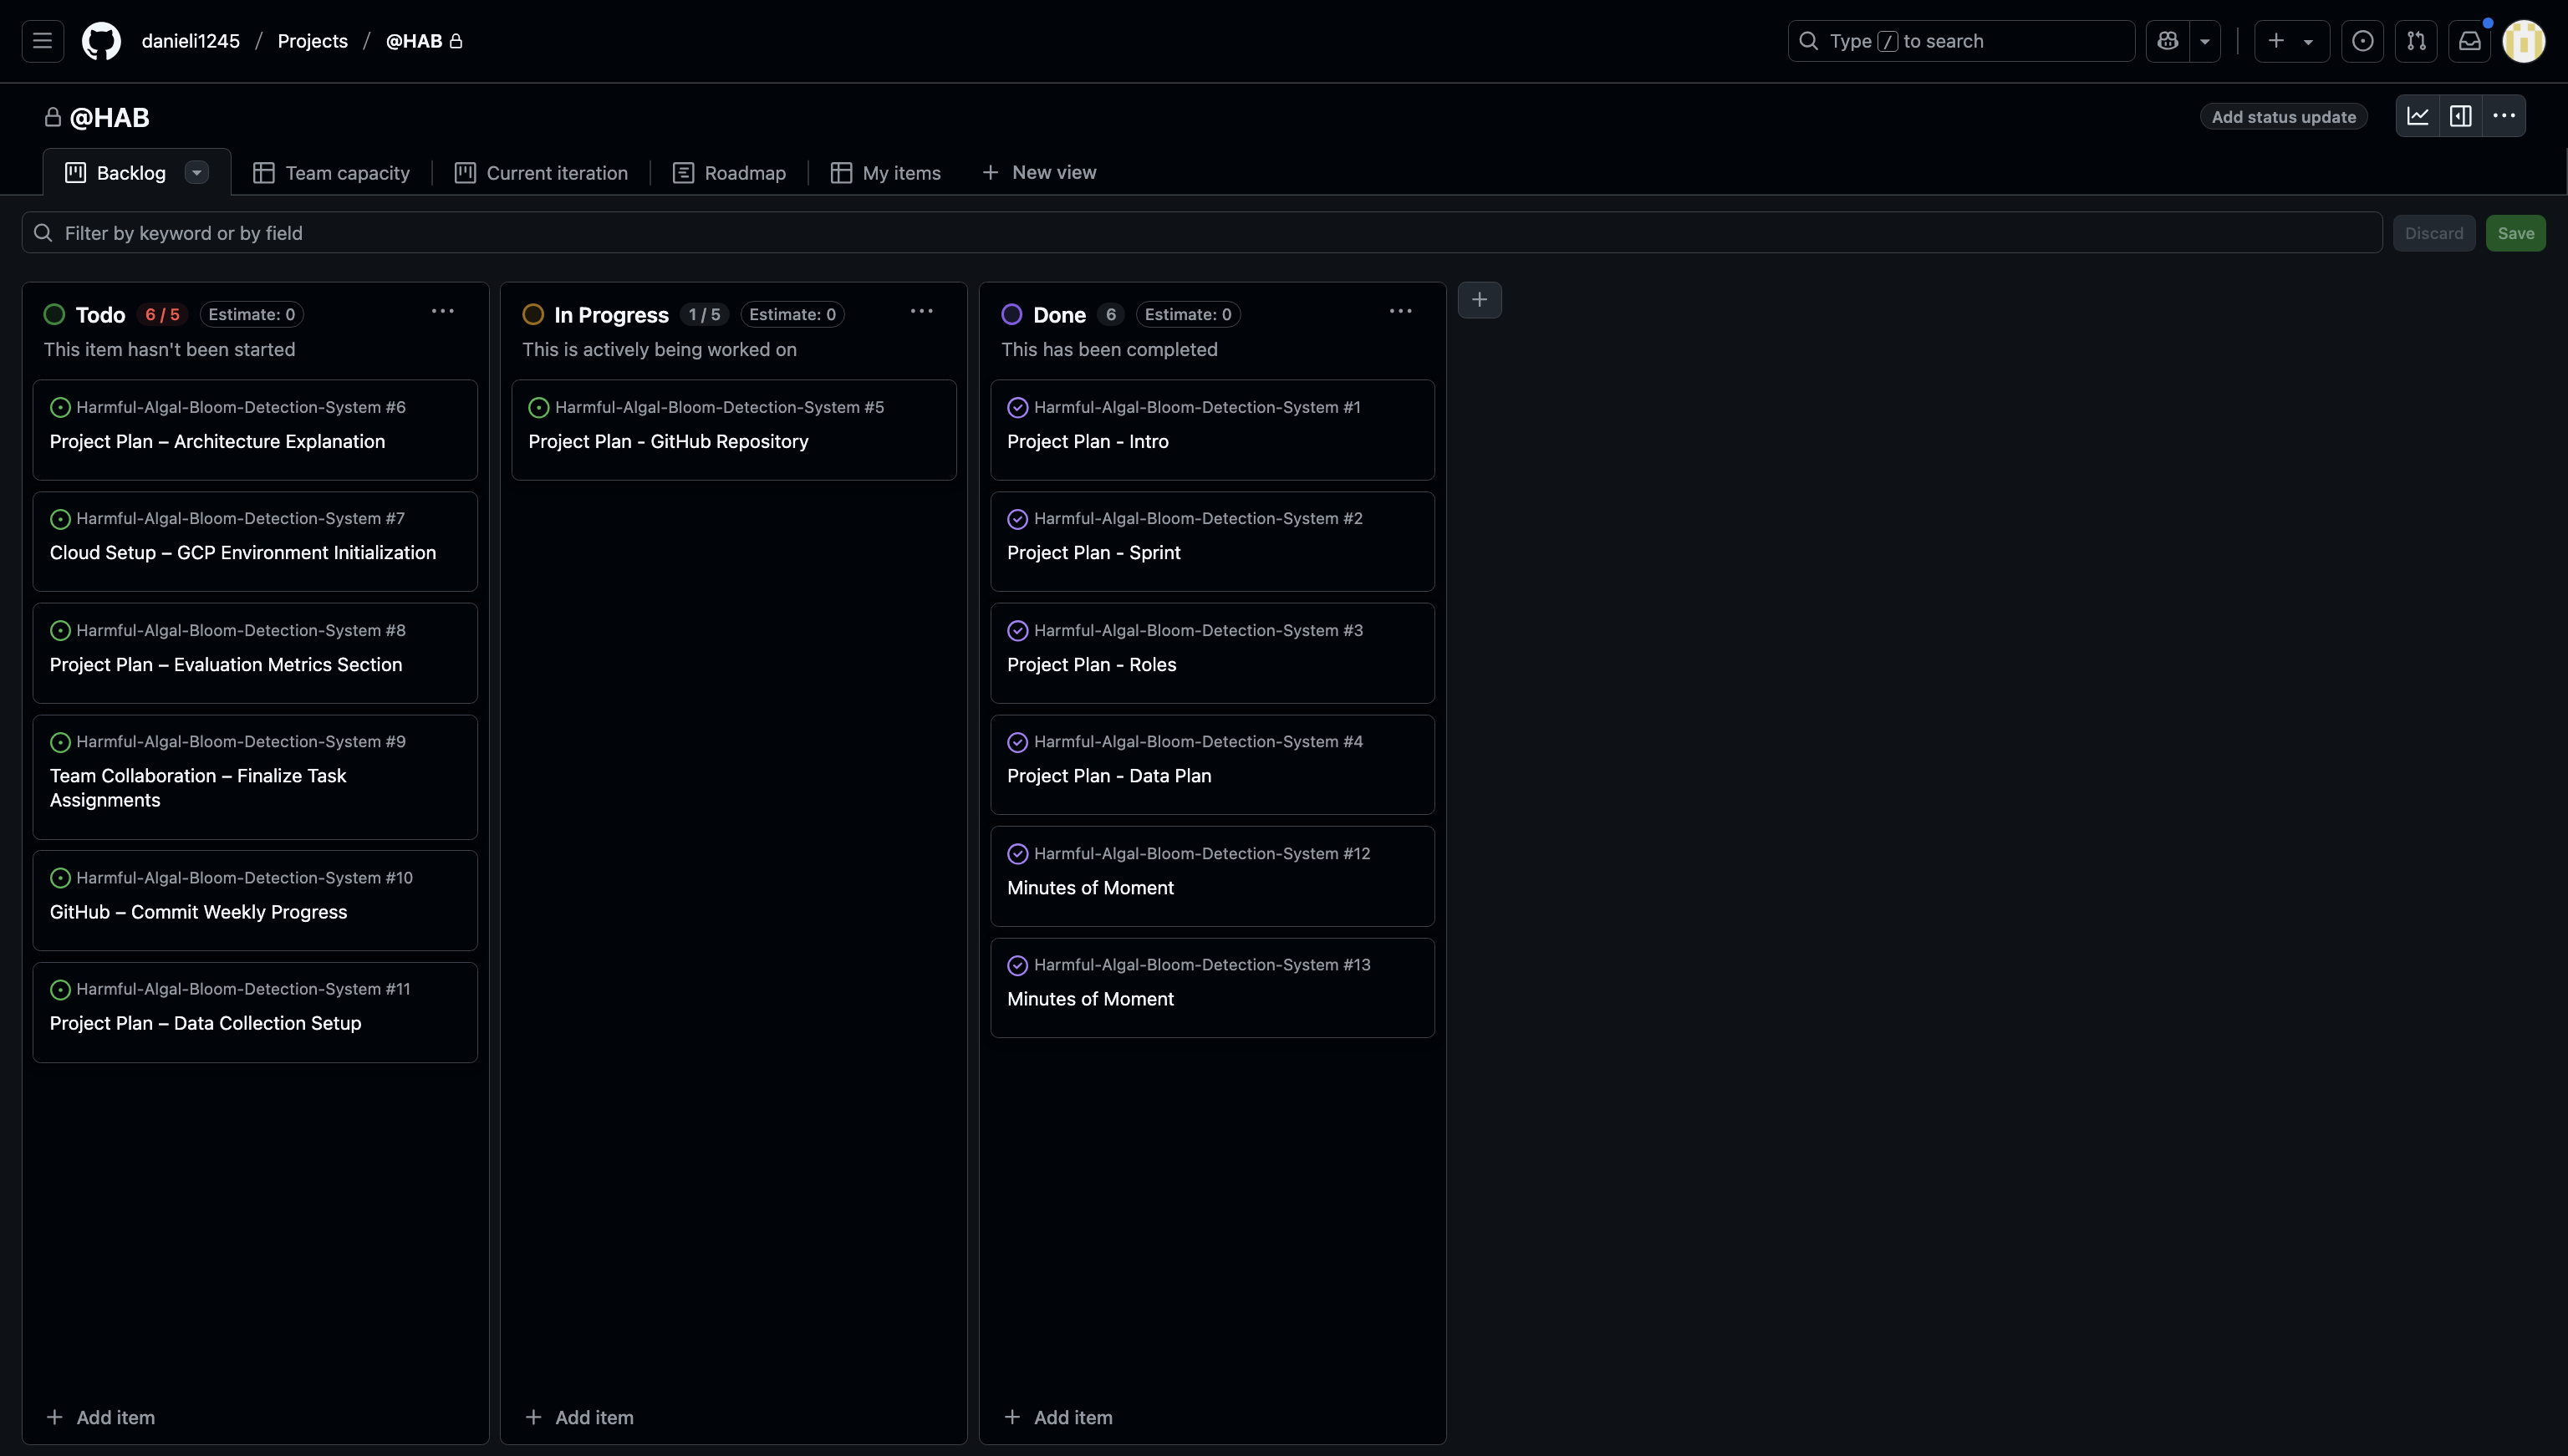
\includegraphics[width=\linewidth]{GithubProject.png}
\captionsetup{width=.8\linewidth} 
\caption[GitHub Projects Board]{GitHub Projects dashboard showing task sprint planning and progress tracking with To Do, In Progress, and Completed items}
\label{fig:github-project}
\end{figure}

\textbf{Accountability:}
\begin{itemize}
    \item \textbf{Sprint Planning:} Tasks are defined and assigned during our meeting planning sessions
    \item \textbf{Progress Tracking:} Daily updates via Whatsapp and status changes on GitHub Projects
    \item \textbf{Blockers:} Issues are brought forward and addressed during the weekly team meetings
\end{itemize}

%%------------------------------------------------
\section{Current Status and Future Directions}
%%------------------------------------------------

The project is currently in the data acquisition phase. This document presents the foundational strategy for HAB detection implementation. The approach will be refined and optimized based on discoveries made during the data collection and initial experimentation phases.

The methodology will be continuously evaluated and improved as new insights emerge from the data analysis process.



%%------------------------------------------------
% End 
%%------------------------------------------------


\bibliographystyle{plain}
\bibliography{references} 

\end{document}
